\begin{name}
	{NGUYÊN HÀM - TÍCH PHÂN}
	{KT ỨNG DỤNG NGUYÊN HÀM - TÍCH PHÂN}
	{\tentruong}
	{\thoigian}
\end{name}
\setcounter{ex}{0}\setcounter{bt}{0}

\Opensolutionfile{ans}[ans/ans-2-C4B13-D1]
\TN
\begin{ex}%[Dự án 2025 - đề cấu trúc mới, Hung Doan]%[2D4N3-1]
	Cho hàm số $y=f(x)$ liên tục trên đoạn $[a;b]$. Khi đó, diện tích hình phẳng giới hạn bởi đồ thị của hàm số $y=f(x)$, trục hoành và hai đường thẳng $x=a$, $x=b$ được tính bởi công thức.
	\choice
	{$S=\pi \displaystyle\int \limits_a^b f(x)\mathrm{\,d}x$}
	{$S=\pi \displaystyle\int \limits_a^b |f(x)|\mathrm{\,d}x$}
	{$S=\displaystyle\int \limits_a^b f(x)\mathrm{\,d}x$}
	{\True $S=\displaystyle\int \limits_a^b |f(x)|\mathrm{\,d}x$}
	\loigiai{
		Công thức diện tích hình phẳng giới hạn bởi đồ thị của hàm số $y=f(x)$, trục hoành và hai đường thẳng $x=a$, $x=b$ là $S=\displaystyle\int \limits_a^b |f(x)|\mathrm{\,d}x$.
	}
\end{ex}
\begin{ex}%[Dự án 2025 - đề cấu trúc mới, Hung Doan]%[2D4N3-1]
	Diện tích hình phẳng giới hạn bởi đồ thị của hàm số $y=x^2-4x+3$, trục hoành và hai đường thẳng $x=0$, $x=3$ là
	\choice
	{$S=\pi \displaystyle\int \limits_0^3 \left(x^2-4x+3\right)\mathrm{\,d}x$}
	{$S=\pi \displaystyle\int \limits_0^3 \left|x^2-4x+3\right|\mathrm{\,d}x$}
	{$S=\displaystyle\int \limits_0^3 \left(x^2-4x+3\right)\mathrm{\,d}x$}
	{\True $S=\displaystyle\int \limits_0^3 \left|x^2-4x+3\right|\mathrm{\,d}x$}
	\loigiai{
		Diện tích hình phẳng giới hạn bởi đồ thị của hàm số $y=x^2-4x+3$, trục hoành và hai đường thẳng $x=0$, $x=3$ là
		$$S=\displaystyle\int \limits_0^3 \left|x^2-4x+3\right|\mathrm{\,d}x.$$
	}
\end{ex}
\begin{ex}%[Dự án 2025 - đề cấu trúc mới, Hung Doan]%[2D4N3-1]
	Cho hai hàm số $y=f(x)$, $y=g(x)$ liên tục trên đoạn $[a;b]$. Khi đó, diện tích hình phẳng giới hạn bởi đồ thị của hai hàm số $y=f(x)$, $y=g(x)$ và hai đường thẳng $x=a$, $x=b$ được tính bởi công thức
	\choice
	{$S=\pi \displaystyle\int \limits_a^b [f(x)-g(x)]\mathrm{\,d}x$}
	{$S=\displaystyle\int \limits_a^b \left|f^2(x)-g^2(x)\right|\mathrm{\,d}x$}
	{\True $S=\displaystyle\int \limits_a^b |f(x)-g(x)|\mathrm{\,d}x$}
	{$S=\pi ^2\displaystyle\int \limits_a^b [f(x)-g(x)]\mathrm{\,d}x$}
	\loigiai{
		Diện tích hình phẳng giới hạn bởi đồ thị của hai hàm số $y=f(x)$, $y=g(x)$ và hai đường thẳng $x=a$, $x=b$ là
		$$S=\displaystyle\int \limits_a^b |f(x)-g(x)|\mathrm{\,d}x.$$
	}
\end{ex}
\begin{ex}%[Dự án 2025 - đề cấu trúc mới, Hung Doan]%[2D4N3-1]
	\immini{Cho hàm số $y=f(x)$ có đồ thị như hình vẽ. Diện tích $S$ của hình phẳng trong phần gạch sọc được tính theo công thức
		\choice
		{$S=-\displaystyle\int \limits_a^b f(x)\mathrm{d}x-\displaystyle\int \limits_b^c f(x)\mathrm{d}x$}
		{$S=\displaystyle\int \limits_a^c f(x)\mathrm{d}x$}
		{$S=\displaystyle\int \limits_a^b f(x)\mathrm{d}x+\displaystyle\int \limits_b^c f(x)\mathrm{d}x$}
		{\True $S=-\displaystyle\int \limits_a^b f(x)\mathrm{d}x+\displaystyle\int \limits_b^c f(x)\mathrm{d}x$}}{
		\begin{tikzpicture}[scale=1, font=\footnotesize, line join=round, line cap=round, >=stealth]
			\def\xt{-2.5} \def\xp{3} \def\yt{3.5} \def\yd{-1.5}
			\draw[->, line width=0.8pt](\xt, 0)--(\xp, 0) node[below]{$x$};
			\draw[->, line width=0.8pt](0,\yd)--(0,\yt) node[left]{$y$};
			\node at (0, 0) [below left]{$O$};
			\clip(\xt+0.1,\yd+0.1) rectangle(\xp-0.1,\yt-0.1);
			\draw[smooth,samples=300] plot(\x,{-0.5*(\x)^3+0.2*(\x)^2+2*(\x)+1});
			\node at (-2, 2) [right]{$y=f(x)$};
			\draw[fill=black](-1.423,0) circle (.04)+(-135:.25) node{$a$};
			\draw[fill=black](-0.584,0) circle (.04)+(100:.25) node{$b$};
			\draw[fill=black](2.41,0) circle (.04)+(-135:.25) node{$c$};
			\fill[pattern=north east lines,smooth] (-1.423,0)--plot[domain=-1.423:2.41](\x,{-0.5*(\x)^3+0.2*(\x)^2+2*(\x)+1})--(2.41,0)--cycle;
		\end{tikzpicture}
	}
	\loigiai{
		Diện tích $S$ của hình phẳng trong phần gạch sọc được tính theo công thức là
		$$S=-\displaystyle\int \limits_a^b f(x)\mathrm{d}x+\displaystyle\int \limits_b^c f(x)\mathrm{d}x.$$
	}
\end{ex}
\begin{ex}%[Dự án 2025 - đề cấu trúc mới, Hung Doan]%[2D4N3-3]
	Cho hàm số $y=f(x)$ liên tục trên đoạn $[a;b]$. Gọi $D$ là hình phẳng giới hạn bởi đồ thị hàm số $y=f(x)$, trục hoành và hai đường thẳng $x=a$, $x=b$ $(a<b)$. Thể tích khối tròn xoay tạo thành khi quay $D$ quanh trục $Ox$ được tính theo công thức
	\choice
	{$V=\displaystyle\int \limits_a^b f^2(x)\mathrm{\,d}x$}
	{$V=\pi \displaystyle\int \limits_a^b f(x)\mathrm{\,d}x$}
	{$V=\displaystyle\int \limits_a^b |f(x)|\mathrm{\,d}x$}
	{\True $V=\pi \displaystyle\int \limits_a^b f^2(x)\mathrm{\,d}x$}
	\loigiai{
		Thể tích khối tròn xoay tạo thành khi quay $D$ quanh trục $Ox$ được tính theo công thức là
		$$V=\pi \displaystyle\int \limits_a^b f^2(x)\mathrm{\,d}x.$$
	}
\end{ex}
\begin{ex}%[Dự án 2025 - đề cấu trúc mới, Hung Doan]%[2D4N3-1]
	Diện tích hình phẳng giới hạn bởi đồ thị của hai hàm số $y=x^3-3x$, $y=x$ và hai đường thẳng $x=-1$, $x=3$ được xác định bởi công thức
	\choice
	{$S=\displaystyle\int \limits_{-1}^3 \left(x^3-3x+x\right)\mathrm{\,d}x$}
	{$S=\displaystyle\int \limits_{-1}^3 \left(x^3-3x-x\right)\mathrm{\,d}x$}
	{$S=\displaystyle\int \limits_{-1}^3 \left|x^3-3x+x\right|\mathrm{\,d}x$}
	{\True $S=\displaystyle\int \limits_{-1}^3 \left|x^3-4x\right|\mathrm{\,d}x$}
	\loigiai{
		Diện tích hình phẳng giới hạn bởi $y=x^3-3x$, $y=x$ và $x=-1$, $x=3$ là
		$$S=\displaystyle\int \limits_{-1}^3 \left|x^3-3x-x\right|\mathrm{\,d}x=\displaystyle\int \limits_{-1}^3 \left|x^3-4x\right|\mathrm{\,d}x.$$
	}
\end{ex}
\begin{ex}%[Dự án 2025 - đề cấu trúc mới, Hung Doan]%[2D4N3-1]
	\immini{Cho hàm số $f(x)$ liên tục trên $\mathbb{R}$. Gọi $S$ là diện tích hình phẳng giới hạn bởi các đường $y=f(x)$, $y=0$,$ x=-1$, $x=2$ (như hình vẽ bên). Mệnh đề nào dưới đây đúng?
		\choice
		{$S=-\displaystyle\int \limits_{-1}^1 f(x)\mathrm{\,d}x+\displaystyle\int \limits_1^2 f(x)\mathrm{\,d}x$}
		{$S=\displaystyle\int \limits_{-1}^1 f(x) \mathrm{\,d}x+\displaystyle\int \limits_1^2 f(x) \mathrm{\,d}x$}
		{\True $S=\displaystyle\int \limits_{-1}^1 f(x) \mathrm{\,d}x-\displaystyle\int \limits_1^2 f(x) \mathrm{\,d}x$}
		{$S=-\displaystyle\int \limits_{-1}^1 f(x) \mathrm{\,d}x-\displaystyle\int \limits_1^2 f(x) \mathrm{\,d}x$}}{
		\begin{tikzpicture}[scale=1, font=\footnotesize, line join=round, line cap=round, >=stealth]
			\def\xt{-1.5} \def\xp{3} \def\yt{3} \def\yd{-1.5}
			\draw[->, line width=0.8pt](\xt, 0)--(\xp, 0) node[below]{$x$};
			\draw[->, line width=0.8pt](0,\yd)--(0,\yt) node[left]{$y$};
			\node at (0, 0) [below left]{$O$};
			\clip(\xt+0.1,\yd+0.1) rectangle(\xp-0.1,\yt-0.1);
			\draw[smooth,samples=300] plot(\x,{(\x)^3-2*(\x)^2-(\x)+2});
			\fill[pattern=north east lines,smooth] (-1,0)--plot[domain=-1:2](\x,{(\x)^3-2*(\x)^2-(\x)+2})--(2,0)--cycle;
			\draw[fill=black](-1,0) circle (.04)+(145:.35) node{$-1$};
			\draw[fill=black](1,0) circle (.04)+(-125:.3) node{$1$};
			\draw[fill=black](2,0) circle (.04)+(-45:.3) node{$2$};
		\end{tikzpicture}
	}
	\loigiai{
		Diện tích hình phẳng giới hạn bởi các đường $y=f(x),y=0,x=-1,x=2$ là
		$$S=\displaystyle\int \limits_{-1}^1 f(x) \mathrm{\,d}x-\displaystyle\int \limits_1^2 f(x) \mathrm{\,d}x.$$
	}
\end{ex}
\begin{ex}%[Dự án 2025 - đề cấu trúc mới, Hung Doan]%[2D4N3-1]
	Diện tích hình phẳng giới hạn bởi đồ thị của hai hàm số $y=x^3+2x+1$, $y=x^3+x+3$ và hai đường thẳng $x=1$, $x=3$ được xác định bởi công thức
	\choice
	{$S=\displaystyle\int \limits_1^3 (2x^3+3x+4)\mathrm{\,d}x$}
	{$S=\displaystyle\int \limits_1^3 (x-2)\mathrm{\,d}x$}
	{\True $S=\displaystyle\int \limits_1^3 |x-2|\mathrm{\,d}x$}
	{$S=\displaystyle\int \limits_1^3 |2x^3+3x+4|\mathrm{\,d}x$}
	\loigiai{
		Diện tích hình phẳng giới hạn bởi $y=x^3+2x+1$, $y=x^3+x+3$, $x=1$, $x=3$ là
		$$S=\displaystyle\int \limits_1^3 \left|x^3+2x+1-(x^3+x+3)\right|\mathrm{\,d}x=\displaystyle\int \limits_1^3 |x-2|\mathrm{\,d}x.$$
	}
\end{ex}
\begin{ex}%[Dự án 2025 - đề cấu trúc mới, Hung Doan]%[2D4H3-1]
	Diện tích hình phẳng giới hạn bởi hai đường $y=x^2+2x$ và $y=-x+4$ bằng
	\choice
	{$\dfrac{13}{2}$}
	{$\dfrac{63}{2}$}
	{$\dfrac{205}{6}$}
	{\True $\dfrac{125}{6}$}
	\loigiai{
		\begin{itemize}
			\item Phương trình hoành độ giao điểm của hai đồ thị hàm số $y=x^2+2x$ và $y=-x+4$ là
			$$x^2+2x=-x+4\Leftrightarrow x^2+3x-4=0\Leftrightarrow \hoac{&x=1\\&x=-4.}$$
			\item Diện tích hình phẳng cần tìm là
			\begin{align*}
				S&=\displaystyle\int \limits_{-4}^1 |x^2+2x-(-x+4)|\mathrm{d}x\\
				&=\displaystyle\int \limits_{-4}^1 |x^2+3x-4|\mathrm{d}x\\
				&=\displaystyle\int \limits_{-4}^1 |x^2+3x-4|\mathrm{d}x\\
				&=\displaystyle\int \limits_{-4}^1 (4-3x-x^2)\mathrm{d}x\\
				&=\left(4x-\dfrac{3}{2}x^2-\dfrac{1}{3}x^3\right)\bigg|^1_{-4}=\dfrac{125}{6}.
			\end{align*}
		\end{itemize}
	}
\end{ex}
\begin{ex}%[Dự án 2025 - đề cấu trúc mới, Hung Doan]%[2D4H3-1]
	Diện tích hình phẳng được giới hạn bởi các đường $y=x^2+x-1$ và $y=x^4+x-1$ là
	\choice
	{$\dfrac{8}{15}$}
	{$\dfrac{7}{15}$}
	{$\dfrac{2}{5}$}
	{\True $\dfrac{4}{15}$}
	\loigiai{
		\begin{itemize}
			\item Phương trình hoành độ giao điểm của $y=x^2+x-1$ và $y=x^4+x-1$ là
			$$x^2+x-1=x^4+x-1 \Leftrightarrow x^2-x^4=0\Leftrightarrow \hoac{&x=0\\&x=1\\&x=-1.}$$
			\item Diện tích hình phẳng cần tìm là
			\begin{align*}
				S&=\displaystyle\int \limits_{-1}^1 |x^2-x^4|\mathrm{d}x\\
				&=\displaystyle\int \limits_{-1}^0 |x^2-x^4|\mathrm{d}x+\displaystyle\int \limits_0^1 |x^2-x^4|\mathrm{d}x\\
				&=\left|\displaystyle\int \limits_{-1}^0 (x^2-x^4)\mathrm{d}x\right|+\left|\displaystyle\int \limits_0^1 (x^2-x^4)\mathrm{d}x\right|\\
				&=\left|\left(\dfrac{x^3}{3}-\dfrac{x^5}{5}\right)\bigg|^0_{-1}\right|+\left|\left(\dfrac{x^3}{3}-\dfrac{x^5}{5}\right)\bigg|^1_0 \right|\\
				&=\dfrac{2}{15}+\dfrac{2}{15}=\dfrac{4}{15}.
			\end{align*}
	\end{itemize}}
\end{ex}
\begin{ex}%[Dự án 2025 - đề cấu trúc mới, Hung Doan]%[2D4H3-3]
	Tính thể tích khối tròn xoay được tạo bởi hình phẳng giới hạn bởi đồ thị hàm số $y=3x-x^2$ và trục hoành khi quay quanh trục hoành.
	\choice
	{$\dfrac{85\pi}{7}$}
	{$\dfrac{8\pi}{7}$}
	{\True $\dfrac{81\pi}{10}$}
	{$\dfrac{41\pi}{7}$}
	\loigiai{
		Phương trình hoành độ giao điểm của đồ thị hàm số $y=3x-x^2$ và trục hoành là $$3x-x^2=0\Leftrightarrow \hoac{&x=0\\&x=3.}$$
		Thể tích của khối tròn xoay là $V=\pi \displaystyle\int \limits_0^3 (3x-x^2)^2\mathrm{\,d}x=\dfrac{81\pi}{10}$.}
\end{ex}
\begin{ex}%[Dự án 2025 - đề cấu trúc mới, Hung Doan]%[2D4H3-1]
	Giá trị dương của tham số $m$ sao cho diện tích hình phẳng giới hạn bởi đồ thị của hàm số $y=2x+3$ và các đường thẳng $y=0$, $x=0$, $x=m$ bằng $10$ là
	\choice
	{$m=\dfrac{7}{2}$}
	{$m=5$}
	{\True $m=2$}
	{$m=1$}
	\loigiai{
		Vì $m>0$ nên $2x+3>0$, $\forall x\in [0;m]$.\\
		Diện tích hình phẳng giới hạn bởi đồ thị hàm số $y=2x+3$ và các đường thẳng $y=0$, $x=0$, $x=m$ là
		$$S=\displaystyle\int \limits_0^m (2x+3)\mathrm{d}x=(x^2+3x)\bigg|_0^m=m^2+3m.$$
		Theo giả thiết ta có
		\begin{align*}
			S=10&\Leftrightarrow m^2+3m=10\\
			&\Leftrightarrow m^2+3m-10=0\\
			&\Leftrightarrow \hoac{&m=2\\&m=-5}\\
			&\Leftrightarrow m=2\, (\text{do} m>0).
		\end{align*}
	}
\end{ex}
\Closesolutionfile{ans}
% \indapan{6}{ans/ans-2-C4B13-D1}
\TNTF
\Opensolutionfile{ans}[ans/ans-2-C4B13-D1-DS]
\begin{ex}%[Dự án 2025 - đề cấu trúc mới, Hung Doan]%[2D4H3-1]
	\immini[thm]{Cho đồ thị hàm số $y=f(x)$, và hình phẳng $(H)$ được gạch chéo như hình vẽ. Đặt $a=\displaystyle\int \limits_{-1}^0 f(x)\mathrm{d}x $, $b=\displaystyle\int \limits_0^2 f(x)\mathrm{d}x$.
		\choiceTF
		{Hình phẳng $(H)$ được giới hạn bởi các đường $x=-1$, $x=2$, $y=f(x)$}
		{Hình phẳng $(H)$ có diện tích $S=\left|\displaystyle\int \limits_{-1}^2 f(x)\mathrm{d}x\right|$}
		{\True Hình phẳng $(H)$ có diện tích $S=b-a$}
		{\True $\displaystyle\int \limits_{-1}^2 f(x)\mathrm{d}x>0$}}{
		\begin{tikzpicture}[scale=1, font=\footnotesize, line join=round, line cap=round, >=stealth]
			\def\xt{-2} \def\xp{3} \def\yt{5} \def\yd{-1.5}
			\draw[->, line width=0.8pt](\xt, 0)--(\xp, 0) node[below]{$x$};
			\draw[->, line width=0.8pt](0,\yd)--(0,\yt) node[left]{$y$};
			\node at (0, 0) [below left]{$O$};
			\clip(\xt+0.1,\yd+0.1) rectangle(\xp-0.1,\yt-0.1);
			\draw[smooth,samples=300] plot(\x,{0.4*(\x)^3});
			\fill[pattern=north east lines,smooth] (-1,0)--plot[domain=-1:2](\x,{0.4*(\x)^3})--(2,0)--cycle;
			\draw[fill=black](-1,0) circle (.04)+(145:.35) node{$-1$};
			\draw[fill=black](2,0) circle (.04)+(-90:.3) node{$2$};
			\draw (-1,-0.4)--(-1,0) (2,0)--(2,3.2);
			\node at (2, 3.5) [left]{$f(x)$};
		\end{tikzpicture}
	}
	\loigiai{
		\begin{itemchoice}
			\itemch \textbf{Sai}.\\
			Ta có hình phẳng $(H)$ được giới hạn bởi các đường $x=-1$, $x=2$, $y=f(x)$ và trục $Ox$.
			\itemch \textbf{Sai}.\\
			Hình phẳng $(H)$ có diện tích $S=\displaystyle\int \limits_{-1}^2 \left|f(x)\right|\mathrm{d}x$.
			\itemch \textbf{Đúng}.\\
			Hình phẳng $(H)$ có diện tích $S=b-a$.
			\itemch \textbf{Đúng}.\\
			Ta có $b>a$ nên $S>0$ hay $\displaystyle\int \limits_{-1}^2 f(x)\mathrm{d}x>0$.
		\end{itemchoice}
	}
\end{ex}
\begin{ex}%[Dự án 2025 - đề cấu trúc mới, Hung Doan]%[2D4V3-3]
	\immini{Cho đồ thị của hai hàm số $y=f(x)$, $y=g(x)$ và phần tô màu như hình vẽ.
		\choiceTF
		{Phần hình phẳng tô màu được giới hạn bởi các đường $y=f(x)$, $y=g(x)$, $x=-3$, $x=3$}
		{\True Hình phẳng giới hạn bởi $y=f(x)$, trục $Ox$ có diện tích $S_1=\dfrac{32}{3}$}
		{\True Phần hình phẳng tô màu có diện tích $S_2=\dfrac{9}{2}$}
		{Quay hình phẳng tô màu quanh trục $Ox$ ta được khối tròn xoay có thể tích $V=\dfrac{9}{2}\pi $}}{
		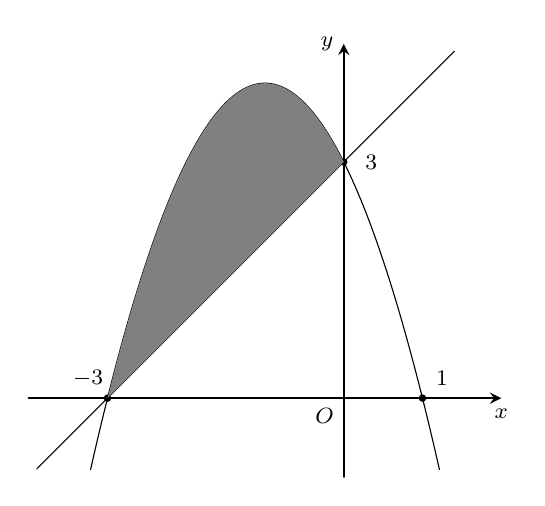
\begin{tikzpicture}[scale=1, font=\footnotesize, line join=round, line cap=round, >=stealth]
			\def\xt{-4} \def\xp{2} \def\yt{4.5} \def\yd{-1}
			\draw[->, line width=0.8pt](\xt, 0)--(\xp, 0) node[below]{$x$};
			\draw[->, line width=0.8pt](0,\yd)--(0,\yt) node[left]{$y$};
			\node at (0, 0) [below left]{$O$};
			\clip(\xt+0.1,\yd+0.1) rectangle(\xp-0.1,\yt-0.1);
			\draw[smooth,samples=300] plot(\x,{-(\x)^2-2*(\x)+3});
			\draw[smooth,samples=300] plot(\x,{(\x)+3});
			\foreach \x/\g in{-3/135,1/45}\draw[fill=black](\x,0) circle (.04)+(\g:.35) node{$\x$};
			\draw[fill=black](0,3) circle (.04)+(0:.35) node{$3$};
			\fill[gray,smooth] (-3,0)--plot[domain=-3:0](\x,{-(\x)^2-2*(\x)+3})--plot[domain=-3:0](\x,{(\x)+3})--cycle;
		\end{tikzpicture}
	}
	\loigiai{
		\begin{itemchoice}
			\itemch \textbf{Sai}.\\
			Phần hình phẳng tô màu được giới hạn bởi các đường $y=f(x)$, $y=g(x)$, $x=-3$, $x=0$.
			\itemch \textbf{Đúng}.\\
			Từ đồ thị suy ra $f(x)=-x^2-2x+3$, $g(x)=x+3$.\\
			Suy ra diện tích $S_1=\displaystyle\int \limits_{-3}^1 \left(-x^2-2x+3\right)\mathrm{d}x=\dfrac{32}{3}$.
			\itemch \textbf{Đúng}.\\
			Phần hình phẳng tô màu có diện tích $S_2=\displaystyle\int \limits_{-3}^0 \left(f(x)-g(x)\right)\mathrm{d}x=\dfrac{9}{2}$.
			\itemch \textbf{Sai}.\\
			Quay hình phẳng tô màu quanh trục $Ox$ ta được khối tròn xoay có thể tích
			$$\begin{aligned}
				V&=\pi \displaystyle\int \limits_{-3}^0 \left[(-x^2-2x+3)^2-(x+3)^2\right]\mathrm{d}x\\
				&=\pi \displaystyle\int \limits_{-3}^0 \left(x^4+4x^3-3x^2-18x\right)\mathrm{d}x\\
				&=\pi \left(\dfrac{x^5}{5}+x^4-x^3-9x^2\right)\bigg|_{-3}^0=\dfrac{108\pi }{5}.
			\end{aligned}$$
		\end{itemchoice}
	}
\end{ex}
\begin{ex}%[Dự án 2025 - đề cấu trúc mới, Hung Doan]%[2D4V3-1]
	Cho hàm số $y=f(x)$ có đồ thị $y=f'(x)$ cắt trục $Ox$ tại ba điểm có hoành độ $a<b<c$ như hình vẽ bên dưới.
	\begin{center}
		\begin{tikzpicture}[scale=1, font=\footnotesize, line join=round, line cap=round, >=stealth]
			\def\xt{-0.5} \def\xp{5} \def\yt{2} \def\yd{-2.5}
			\draw[->](\xt, 0)--(\xp, 0) node[below]{$x$};
			\draw[->](0,\yd)--(0,\yt) node[left]{$y$};
			\node at (0, 0) [below left]{$O$};
			\clip(\xt+0.1,\yd+0.1) rectangle(\xp-0.1,\yt-0.1);
			\draw[smooth,samples=300] plot(\x,{((\x)-1)*((\x)-2)*((\x)-4)});
			\fill (1,0) node[above left]{$a$} circle (1pt);
			\fill (2,0) node[above right]{$b$} circle (1pt);
			\fill (4,0) node[above left]{$c$} circle (1pt);
			\fill[pattern=north east lines,smooth] (1,0)--plot[domain=1:4](\x,{((\x)-1)*((\x)-2)*((\x)-4)})--(4,0)--cycle;
		\end{tikzpicture}
	\end{center}
	\choiceTF
	{\True Hình phẳng gạch sọc được giới hạn bởi các đường $y=f'(x)$ và trục $Ox$}
	{Diện tích hình phẳng gạch sọc $S=\displaystyle\int \limits_a^b f(x)\mathrm{d}x-\displaystyle\int \limits_b^c f(x)\mathrm{d}x$}
	{$\displaystyle\int \limits_a^b f'(x)\mathrm{d}x<\displaystyle\int \limits_b^c f'(x)\mathrm{d}x$}
	{\True $f(b)>f(a)>f(c)$}
	\loigiai{
		\begin{itemchoice}
			\itemch \textbf{Đúng}.\\
			Hình phẳng gạch sọc được giới hạn bởi các đường $y=f'(x)$ và trục $Ox$.
			\itemch \textbf{Sai}.\\
			Diện tích hình phẳng gạch sọc phải là $S=\displaystyle\int \limits_a^b f'(x)\mathrm{d}x-\displaystyle\int \limits_b^c f'(x)\mathrm{d}x$.
			\itemch \textbf{Sai}.
			\begin{center}
				\begin{tikzpicture}[scale=1, font=\footnotesize, line join=round, line cap=round, >=stealth]
					\def\xt{-0.5} \def\xp{5} \def\yt{2} \def\yd{-2.5}
					\draw[->](\xt, 0)--(\xp, 0) node[below]{$x$};
					\draw[->](0,\yd)--(0,\yt) node[left]{$y$};
					\node at (0, 0) [below left]{$O$};
					\clip(\xt+0.1,\yd+0.1) rectangle(\xp-0.1,\yt-0.1);
					\draw[smooth,samples=300] plot(\x,{((\x)-1)*((\x)-2)*((\x)-4)});
					\fill (1,0) node[above left]{$a$} circle (1pt);
					\fill (2,0) node[above right]{$b$} circle (1pt);
					\fill (4,0) node[above left]{$c$} circle (1pt);
					\fill[pattern=north east lines,smooth] (1,0)--plot[domain=1:4](\x,{((\x)-1)*((\x)-2)*((\x)-4)})--(4,0)--cycle;
					\node at (1.5, -0.1) [above]{$S_1$};
					\node at (3, -0.5) [below]{$S_2$};
				\end{tikzpicture}
			\end{center}
			Ta có diện tích $S_1=\displaystyle\int \limits_a^b f'(x)\mathrm{d}x$, diện tích $S_2=-\displaystyle\int \limits_b^c f'(x)\mathrm{d}x$.\\
			Từ hình vẽ ta có $S_1<S_2 \Leftrightarrow \displaystyle\int \limits_a^b f'(x)\mathrm{d}x<-\displaystyle\int \limits_b^c f'(x)\mathrm{d}x$.\\
			\itemch \textbf{Đúng}.\\
			Ta có $\displaystyle\int \limits_a^b f'(x)\mathrm{d}x<-\displaystyle\int \limits_b^c f'(x)\mathrm{d}x\Leftrightarrow f(b)-f(a)<f(b)-f(c) \Leftrightarrow f(a)>f(c)$.\\
			Mặt khác, từ đồ thị hàm $f'(x)$ ta có bảng biến thiên
			\begin{center}
				
\begin{tikzpicture}
					\tkzTabInit[nocadre=true,lgt=1.5,espcl=3,deltacl=.55]
					{$x$/0.7, $f'(x)$/0.7, $f(x)$/2}
					{$-\infty$,$a$,$b$,$c$,$+\infty$}
					\tkzTabLine{,-,$0$,+,$0$,-,$0$,+,}
					\tkzTabVar{+/$+\infty$,-/$f(a)$,+/$f(b)$,-/$f(c)$,+/$+\infty$}	
				\end{tikzpicture}
			\end{center}
			Suy ra $f(b)$ lớn hơn $f(a)$ và $f(c)$.\\
			Vậy $f(b)>f(a)>f(c)$.
		\end{itemchoice}
	}
\end{ex}
\begin{ex}%[Dự án 2025 - đề cấu trúc mới, Hung Doan]%[2D4H3-1]
	\immini[thm]{Cho hình vuông $ABCD$ tâm $O$, độ dài cạnh là $4$ cm. Đường cong $BOC$ là một phần của parabol đỉnh $O$ chia hình vuông thành hai hình phẳng có diện tích lần lượt là $S_1$ và $S_2$ (tham khảo hình vẽ).
		\choiceTF
		{Diện tích hình phẳng $S_1=4$}
		{Diện tích hình phẳng $S_2=12$}
		{\True $S_2=2S_1$}
		{$S_2=3S_1$}}{
		\begin{tikzpicture}[scale=1, font=\footnotesize, line join=round, line cap=round, >=stealth]
			\node at (0, 0) [below]{$O$};
			\node at (0, 2.2) {$4$\,cm};
			\node at (2.4, 0) {$4$\,cm};
			\node at (0,1) {$S_1$};
			\node at (0,-1) {$S_2$};
			\fill (-2,-2) node[below left]{$A$};
			\fill (-2,2) node[above left]{$B$};
			\fill (2,2) node[above right]{$C$};
			\fill (2,-2) node[below right]{$D$};
			\clip(-2.1,-2.1) rectangle(2.1,2);
			\draw[smooth,samples=300] plot(\x,{0.5*(\x)^2});
			\draw (2,2)--(2,-2)--(-2,-2)--(-2,2)--(2,2);
		\end{tikzpicture}
		
	}
	\loigiai{
		Gắn hệ trục toạ độ như hình vẽ
		\begin{center}
			\begin{tikzpicture}[scale=1, font=\footnotesize, line join=round, line cap=round, >=stealth]
				\draw[->](-3, 0)--(3, 0) node[below]{$x$};
				\draw[->](0,-3)--(0,3) node[left]{$y$};
				\node at (0, 0) [below left]{$O$};
				\fill (-2,-2) node[below left]{$A$};
				\fill (-2,2) node[above left]{$B$};
				\fill (2,2) node[above right]{$C$};
				\fill (2,-2) node[below right]{$D$};
				\fill (-2,0) node[below left]{$-2$} circle (1pt);
				\fill (0,2) node[above left]{$2$};
				\fill (2,0) node[above right]{$2$};
				\fill (0,-2) node[below right]{$-2$};
				\clip(-2.1,-2.1) rectangle(2.1,2);
				\draw[smooth,samples=300] plot(\x,{0.5*(\x)^2});
				\draw (2,2)--(2,-2)--(-2,-2)--(-2,2)--(2,2);
			\end{tikzpicture}
		\end{center}
		Ta có phương trình parabol $(P)\colon y=\dfrac{1}{2}x^2$.\\
		Suy ra $S_1=\displaystyle\int \limits_{-2}^2 \left(2-\dfrac{1}{2}x^2\right)\mathrm{\,d}x=\dfrac{16}{3}$ (đvdt).\\
		Diện tích hình vuông $ABCD$ là $S_{ABCD}=4^2=16$ (đvdt).\\
		Do đó diện tích $S_2$ là $S_2=S_{ABCD}-S_1=16-\dfrac{16}{3}=\dfrac{32}{3}$ (đvdt).\\
		Vậy tỉ số $\dfrac{S_1}{S_2}=\dfrac{16}{3}\colon \dfrac{32}{3}=\dfrac{1}{2}\Rightarrow S_2=2S_1$.\\
		Khi đó, ta có
		\begin{itemchoice}
			\itemch \textbf{Sai}.
			\itemch \textbf{Sai}.
			\itemch \textbf{Đúng}.
			\itemch \textbf{Sai}.
		\end{itemchoice}
	}
\end{ex}
\Closesolutionfile{ans}
% \indapan{2}{ans/ans-2-C4B13-D1-DS}
\Opensolutionfile{ans}[ans/ans-2-C4B13-D1-KQ]
\TNSA
\begin{ex}%[Dự án 2025 - đề cấu trúc mới, Hung Doan]%[2D4H3-1]
	Tính diện tích hình phẳng giới hạn bởi các đường $y=x^2$, $y=-\dfrac{1}{3}x+\dfrac{4}{3}$ và trục hoành (làm tròn kết quả đến hàng phần trăm).
	\shortans{$1{,}83$}
	\loigiai{
		\begin{center}
			\begin{tikzpicture}[scale=1, font=\footnotesize, line join=round, line cap=round, >=stealth]
				\def\xt{-2} \def\xp{5} \def\yt{3} \def\yd{-1}
				\draw[->, line width=0.8pt](\xt, 0)--(\xp, 0) node[below]{$x$};
				\draw[->, line width=0.8pt](0,\yd)--(0,\yt) node[left]{$y$};
				\node at (0, 0) [below left]{$O$};
				\clip(\xt+0.1,\yd+0.1) rectangle(\xp-0.1,\yt-0.1);
				\draw[ smooth,samples=300] plot(\x,{(\x)^2});
				\draw[ smooth,samples=300] plot(\x,{-1/3*(\x)+4/3});
				\foreach \x in {1,4}
				\draw[shift ={ (\x,0)}]node[below]{$\x$} (0pt,2pt) --(0pt,-2pt);
				\fill[pattern=north east lines,smooth] (0,0)--plot[domain=0:1](\x,{(\x)^2})--(1,0)--cycle;
				\fill[pattern=north east lines,smooth] (1,0)--plot[domain=1:4](\x,{-1/3*(\x)+4/3})--(4,0)--cycle;
				\draw[dashed] (1,0)--(1,1);
			\end{tikzpicture}
		\end{center}
		Phương trình hoành độ giao điểm của các đường là
		\begin{itemize}
			\item $x^2=0\Leftrightarrow x=0$.
			\item $-\dfrac{1}{3}x+\dfrac{4}{3}\Leftrightarrow x=4$.
			\item $x^2=-\dfrac{1}{3}x+\dfrac{4}{3} \Leftrightarrow 3x^2+x-4=0 \Leftrightarrow \hoac{&x=1\\&x=-\dfrac{4}{3}.}$
		\end{itemize}
		Diện tích hình phẳng cần tìm là
		$$S=\displaystyle\int \limits_0^1 x^2\mathrm{d}x+\displaystyle\int \limits_1^4 \left(-\dfrac{1}{3}x+\dfrac{4}{3}\right)\mathrm{d}x =\dfrac{x^3}{3}\bigg|_0^1+\left(-\dfrac{1}{6}x^2+\dfrac{4}{3}x\right)\bigg|_1^4 =\dfrac{11}{6}\approx 1{,}83.$$
	}
\end{ex}
\begin{ex}%[Dự án 2025 - đề cấu trúc mới, Hung Doan]%[2D4V3-1]
	Cho hàm số $y=f(x)$. Hàm số có đồ thị hàm số $y=f'(x)$ như hình vẽ dưới đây.
	\begin{center}
		\begin{tikzpicture}[scale=1, font=\footnotesize, line join=round, line cap=round, >=stealth]
			\def\xt{-2.75} \def\xp{4.75} \def\yt{2.5} \def\yd{-3}
			\draw[->](\xt, 0)--(\xp, 0) node[below]{$x$};
			\draw[->](0,\yd)--(0,\yt) node[left]{$y$};
			\node at (0, 0) [below left]{$O$};
			\node at (-1.5, 1.4) {$y=f'(x)$};
			\foreach \x in {1,4}
			\draw[shift ={ (\x,0)}]node[above]{$\x$} (0pt,2pt) --(0pt,-2pt);
			\draw[shift ={ (-2,0)}]node[above right]{$-2$} (0pt,2pt) --(0pt,-2pt);
			\clip(\xt+0.1,\yd+0.1) rectangle(4,\yt-0.1);
			\draw plot[smooth,tension=0.7] coordinates{(-2.4,2) (-1.2,-1.8) (1,0) (3,-2.5) (4,0)};			
		\end{tikzpicture}
	\end{center}
	Biết diện tích hình phẳng giới hạn bởi trục $Ox$ và đồ thị hàm số $y=f'(x)$ trên đoạn $[-2;1]$ và $[1;4]$ lần lượt bằng $9$ và $12$. Cho biết $f(1)=3$. Tính giá trị biểu thức $P=f(-2)+f(4)$.
	\shortans{$3$}
	\loigiai{
		Ta có $\displaystyle\int \limits_{-2}^1 |f'(x)|\mathrm{d}x=9\Leftrightarrow \displaystyle\int \limits_{-2}^1 f'(x)\mathrm{d}x=-9\Rightarrow f(1)-f(-2)=-9$.\\
		Mà $f(1)=3 \Rightarrow f(-2)=12$.\\
		Ta có $\displaystyle\int \limits_1^4 |f'(x)|\mathrm{d}x=12\Leftrightarrow \displaystyle\int \limits_1^4 f'(x)\mathrm{d}x=-12\Rightarrow f(4)-f(1)=-12$.\\
		Mà $f(1)=3 \Rightarrow f(4)=-9$.\\
		Vậy $P=f(-2)+f(4)=3$.
	}
\end{ex}
\begin{ex}%[Dự án 2025 - đề cấu trúc mới, Hung Doan]%[2D4C3-1]
	Cho hàm số $f(x)=x^3+ax^2+bx+c$ với $a$, $b$, $c$ là các số thực. Biết hàm số $g(x)=f(x)+f'(x)+f''(x)$ có hai giá trị cực trị là $5$ và $2$. Tính diện tích hình phẳng giới hạn bởi đường $y=\dfrac{f(x)}{g(x)+6}$ và $y=1$, kết quả làm tròn đến hàng phần trăm.
	\shortans{$2{,}08$}
	\loigiai{
		Ta có $f'''(x)=6$, khi đó $g'(x)=f'(x)+f''(x)+f'''(x)=f'(x)+f''(x)+6$.\\
		Giả sử $x_1$, $x_2$ ($x_1<x_2$) là hai điểm cực trị của hàm số $g(x)$.\\
		Vì $\lim \limits_{x\to +\infty } g(x)=+\infty $ và $-5$ và $2$ là hai giá trị cực trị của hàm số $g(x)$ nên $\heva{&g(x_1)=2\\&g(x_2)=-5.}$\\
		Phương trình hoành độ giao điểm của $y=\dfrac{f(x)}{g(x)+6}$ và $y=1$ là
		\begin{align*}
			\dfrac{f(x)}{g(x)+6}=1 &\Leftrightarrow g(x)+6=f(x)\\
			&\Leftrightarrow f(x)+f'(x)+f''(x)+6=f(x)\\
			&\Leftrightarrow f'(x)+f''(x)+6=0\\
			&\Leftrightarrow \hoac{&x=x_1\\&x=x_2.} 
		\end{align*}
		Khi đó diện tích hình phẳng cần tìm là
		\begin{align*}
			S&=\displaystyle\int \limits_{x_1}^{x_2} \left|\dfrac{f(x)}{g(x)+6}-1\right|\mathrm{d}x\\
			&=\left|\displaystyle\int \limits_{x_1}^{x_2} \dfrac{f'(x)+f''(x)+6}{g(x)+6}\mathrm{d}x\right|\\
			&=\left|\displaystyle\int \limits_{x_1}^{x_2} \dfrac{g'(x)}{g(x)+6}\mathrm{d}x\right|\\
			&=\left|\ln |g(x)+6|\bigg|_{x_1}^{x_2}\right| \\
			&=\left|\ln |g(x_2)+6|-\ln |g(x_1)+6|\right|\\
			&=\ln 8\approx 2{,}08.
		\end{align*}
	}
\end{ex}
\begin{ex}%[Dự án 2025 - đề cấu trúc mới, Hung Doan]%[2D4V3-2]
	Một viên gạch hoa hình vuông cạnh $40$ cm. Người thiết kế đã sử dụng bốn đường parabol có chung đỉnh tại tâm viên gạch để tạo ra bốn cánh hoa (được tô màu sẫm như hình vẽ bên).
	\begin{center}
		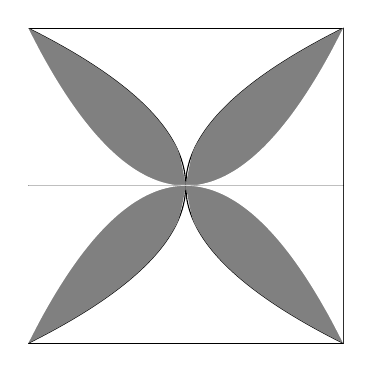
\begin{tikzpicture}[scale=1, font=\footnotesize, line join=round, line cap=round, >=stealth]
			\draw (2,2)--(2,-2)--(-2,-2)--(-2,2)--(2,2);
			\clip(-2,-2) rectangle(2,2);
			\draw[smooth,samples=300] plot(\x,{0.5*(\x)^2});
			\draw[smooth,samples=300] plot(\x,{-0.5*(\x)^2});
			\draw[samples=200,domain=0:2,smooth] plot (\x,{sqrt(2*(\x))});
			\draw[samples=200,domain=0:2,smooth] plot (\x,{-sqrt(2*(\x))});
			\draw[samples=200,domain=-2:0,smooth] plot (\x,{sqrt(-2*(\x))});
			\draw[samples=200,domain=-2:0,smooth] plot (\x,{-sqrt(-2*(\x))});
			\fill[gray,smooth] (-2,0)--plot[domain=-2:0](\x,{-sqrt(-2*(\x))})--(0,0)--cycle;
			\fill[gray,smooth] (-2,0)--plot[domain=-2:0](\x,{sqrt(-2*(\x))})--(0,0)--cycle;
			\fill[gray,smooth] (0,0)--plot[domain=0:2](\x,{-sqrt(2*(\x))})--(2,0)--cycle;
			\fill[gray,smooth] (0,0)--plot[domain=0:2](\x,{sqrt(2*(\x))})--(2,0)--cycle;
			\fill[white,smooth] (-2,0)--plot[domain=-2:2](\x,{-0.5*(\x)^2})--(2,0)--cycle;
			\fill[white,smooth] (-2,0.01)--plot[domain=-2:2](\x,{0.5*(\x)^2})--(2,0.01)--cycle;
		\end{tikzpicture}
	\end{center}
	Diện tích mỗi cánh hoa của viên gạch bằng bằng $\dfrac{a}{b}$ (cm$^2$), với $\dfrac{a}{b}$ là phân số tối giản thì $a$ bằng bao nhiêu?
	\shortans{$400$}
	\loigiai{
		\begin{center}
			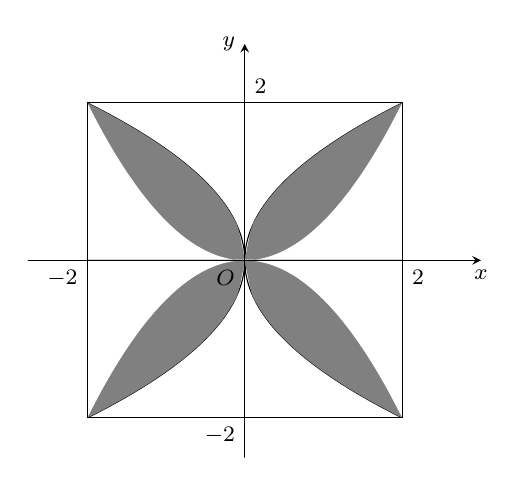
\begin{tikzpicture}[scale=1, font=\footnotesize, line join=round, line cap=round, >=stealth]
				\begin{scope}
					\clip(-2,-2) rectangle(2,2);
					\draw[smooth,samples=300] plot(\x,{0.5*(\x)^2});
					\draw[smooth,samples=300] plot(\x,{-0.5*(\x)^2});
					\draw[samples=200,domain=0:2,smooth] plot (\x,{sqrt(2*(\x))});
					\draw[samples=200,domain=0:2,smooth] plot (\x,{-sqrt(2*(\x))});
					\draw[samples=200,domain=-2:0,smooth] plot (\x,{sqrt(-2*(\x))});
					\draw[samples=200,domain=-2:0,smooth] plot (\x,{-sqrt(-2*(\x))});
					\fill[gray,smooth] (-2,0)--plot[domain=-2:0](\x,{-sqrt(-2*(\x))})--(0,0)--cycle;
					\fill[gray,smooth] (-2,0)--plot[domain=-2:0](\x,{sqrt(-2*(\x))})--(0,0)--cycle;
					\fill[gray,smooth] (0,0)--plot[domain=0:2](\x,{-sqrt(2*(\x))})--(2,0)--cycle;
					\fill[gray,smooth] (0,0)--plot[domain=0:2](\x,{sqrt(2*(\x))})--(2,0)--cycle;
					\fill[white,smooth] (-2,0)--plot[domain=-2:2](\x,{-0.5*(\x)^2})--(2,0)--cycle;
					\fill[white,smooth] (-2,0.01)--plot[domain=-2:2](\x,{0.5*(\x)^2})--(2,0.01)--cycle;
				\end{scope}
				\draw[->](-2.75, 0)--(3, 0) node[below]{$x$};
				\draw[->](0,-2.5)--(0,2.75) node[left]{$y$};
				\node at (0, 0) [below left]{$O$};
				\draw[shift ={ (-2,0)}]node[below left]{$-2$} (0pt,2pt) --(0pt,-2pt);
				\draw[shift ={ (2,0)}]node[below right]{$2$} (0pt,2pt) --(0pt,-2pt);
				\draw[shift ={ (0,2)}]node[above right]{$2$} (2pt,0pt) --(-2pt,0pt);
				\draw[shift ={ (0,-2)}]node[below left]{$-2$} (2pt,0pt) --(-2pt,0pt);
				\draw[smooth] (2,2)--(2,-2)--(-2,-2)--(-2,2)--(2,2);
			\end{tikzpicture}
		\end{center}
		Chọn hệ tọa độ như hình vẽ ($1$ đơn vị trên trục bằng $10$ cm=$1$ dm), các cánh hoa tạo bởi các đường parabol có phương trình $y=\dfrac{x^2}{2}$, $y=-\dfrac{x^2}{2}$, $x=-\dfrac{y^2}{2}$, $x=\dfrac{y^2}{2}$.\\
		Diện tích một cánh hoa (nằm trong góc phần tư thứ nhất) bằng diện tích hình phẳng giới hạn bởi hai đồ thị hàm số $y=\dfrac{x^2}{2}$, $y=\sqrt{2x}$ và hai đường thẳng $x=0$; $x=2$.\\
		Do đó diện tích một cánh hoa bằng
		\begin{align*}
			\displaystyle\int \limits_0^2 \left(\sqrt{2x}-\dfrac{x^2}{2}\right)\mathrm{d}x &=\left(\dfrac{2\sqrt{2}}{3}\sqrt{(2x)^3}-\dfrac{x^3}{6}\right)\bigg|\bigg|_0^2\\
			&=\dfrac{4}{3}(\text{dm}^2)=\dfrac{400}{3}\,(\text{cm}^2).
		\end{align*}
		Suy ra $a=400$.
	}
\end{ex}
\begin{ex}%[Dự án 2025 - đề cấu trúc mới, Hung Doan]%[2D4C3-2]
	\immini[thm]{Một bức tường lớn kích thức $8$m $\times$ $8$m trước đại sảnh của một tòa biệt thự được sơn các loại sơn đặc biệt. Người ta vẽ hai nửa đường tròn đường kính $AD$, $AB$ cắt nhau tại $H$; đường tròn tâm $D$, bán kính $AD$, cắt nửa đường tròn đường kính $AB$ tại $K$. Biết tam giác cong $AHK$ được sơn màu xanh và các phần còn lại được sơn màu trắng (như hình vẽ) và một mét vuông sơn trắng, sơn xanh lần lượt có giá là $1$ triệu đồng và $1{,}5$ triệu đồng. Số tiền phải trả là bao nhiêu triệu đồng? (làm tròn đến hàng triệu).}{
		\begin{tikzpicture}[scale=1, font=\footnotesize, line join=round, line cap=round, >=stealth]
			\begin{scope}
				\clip (0,0) rectangle (4,4);
				\fill[pattern=north east lines,smooth] (0,0)--plot[domain=0:4](\x,{sqrt(16-(\x)^2)})--(4,0)--cycle;
				\fill[white,smooth] (0,0)--plot[domain=0:4](\x,{4-sqrt(4*(\x)-(\x)^2)})--(4,0)--cycle;
				\draw[fill=white,samples=200,domain=0:4,smooth] (0,2) circle (2);
				\draw[samples=200,domain=0:4,smooth,variable=\x] plot (\x,{sqrt(16-(\x)^2)});
				\draw[samples=200,domain=0:4,smooth,variable=\x] plot (\x,{4-sqrt(4*(\x)-(\x)^2)});
				%\draw[samples=200,domain=0:4,smooth] (0,2) circle (2);
			\end{scope}
			\draw (0,0)rectangle (4,4);
			\node at (0, 2) [left]{$8$};
			\node at (2,0) [below]{$8$};
			\fill (0,4) node[above left]{$A$} circle(1pt);
			\fill (0,0) node[below left]{$B$} circle(1pt);
			\fill (4,0) node[below right]{$C$} circle(1pt);
			\fill (4,4) node[above right]{$D$} circle(1pt);
			\fill (2,2) node[below left]{$H$} circle(1pt);
			\fill (3.2,2.4) node[below]{$K$} circle(1pt);
			\draw (0,0)rectangle (0.2,0.2);
			\draw (0,4)rectangle (0.2,3.8);
			\draw (4,0)rectangle (3.8,0.2);
			\draw (4,4)rectangle (3.8,3.8);
		\end{tikzpicture}
	}
	\shortans{$67$}
	\loigiai{
		Chọn hệ toạ độ ${Oxy}$ như hình vẽ sau
		\begin{center}
			\begin{tikzpicture}[scale=1, font=\footnotesize, line join=round, line cap=round, >=stealth]
				\begin{scope}
					\clip (0,0) rectangle (4,4);
					\fill[pattern=north east lines,smooth] (0,0)--plot[domain=0:4](\x,{sqrt(16-(\x)^2)})--(4,0)--cycle;
					\fill[white,smooth] (0,0)--plot[domain=0:4](\x,{4-sqrt(4*(\x)-(\x)^2)})--(4,0)--cycle;
					\draw[fill=white,samples=200,domain=0:4,smooth] (0,2) circle (2);
					\draw[samples=200,domain=0:4,smooth,variable=\x] plot (\x,{sqrt(16-(\x)^2)});
					\draw[samples=200,domain=0:4,smooth,variable=\x] plot (\x,{4-sqrt(4*(\x)-(\x)^2)});
					%\draw[samples=200,domain=0:4,smooth] (0,2) circle (2);
				\end{scope}
				\draw (0,0)rectangle (4,4);
				\node at (0, 2) [left]{$8$};
				\node at (2,0) [below]{$8$};
				\fill (0,4) node[above left]{$A$} circle(1pt);
				\fill (0,0) node[below left]{$B$} circle(1pt);
				\fill (4,0) node[below right]{$C$} circle(1pt);
				\fill (4,4) node[above right]{$D$} circle(1pt);
				\fill (2,2) node[below left]{$H$} circle(1pt);
				\fill (3.2,2.4) node[below]{$K$} circle(1pt);
				\draw (0,0)rectangle (0.2,0.2);
				\draw (0,4)rectangle (0.2,3.8);
				\draw (4,0)rectangle (3.8,0.2);
				\draw (4,4)rectangle (3.8,3.8);
				\draw[->](-0.5, 0)--(5, 0) node[below]{$x$};
				\draw[->](0,-0.5)--(0,5) node[left]{$y$};
				\node at (0, 0) [above left]{$O$};
				\draw[dashed] (2,2)--(2,3.4641)node[above]{$E$};
			\end{tikzpicture}
		\end{center}
		Dễ thấy cung $AB$ có phương trình $y=f(x)=8-\sqrt{16-(x-4)^2}$; cung $AH$ có phương trình $y=g(x)=4+\sqrt{16-x^2}$; cung $AC$ có phương trình $y=h(x)=\sqrt{64-x^2}$ và tọa độ các điểm $H(4;4)$ và $K\left(6{,}4;\dfrac{24}{5}\right)$.\\
		Diện tích tam giác $AHK$ là
		\begin{align*}
			S&=S_{AHE}+S_{HEX}\\
			&=\displaystyle\int \limits_0^4 (\sqrt{64-x^2}-4-\sqrt{16-x^2})\mathrm{d}x+\displaystyle\int \limits_4^{6\cdot 4} (\sqrt{64-x^2}-8+\sqrt{16-(x-4)^2})\mathrm{d}x\\
			&\approx 6,25\,5085\,231.
		\end{align*}
		Số tiền cần trả là $S\cdot 1{,}5+(8^2-S)\cdot 1=67{,}12\,754\,262$.\\
		Vậy số tiền cần trả là $67$ (triệu đồng).
	}
\end{ex}
\begin{ex}%[Dự án 2025 - đề cấu trúc mới, Hung Doan]%[2D4V3-5]
	\immini{Một cốc có hình dạng tròn xoay và kích thước như hình vẽ, thiết diện dọc của mặt bên trong cốc (bổ dọc cốc thành $2$ phần bằng nhau) là một đường Parabol. Tính thể tích tối đa mà cốc có thể chứa được (kết quả làm tròn đến chữ số hàng đơn vị).}{
		\definecolor{almond}{rgb}{0.94, 0.87, 0.8}%màu ly
		\definecolor{anti-flashwhite}{rgb}{0.95, 0.95, 0.96}%màu miệng ly
		\begin{tikzpicture}[line join=round, line cap=round,scale=0.5,transform shape,line width=.3mm]
			
			\tikzset{co_vat/.pic={
					\path 
					(1.85,4)coordinate (A)			
					(-1.85,4) coordinate (B)	
					(-3,3)coordinate (C)
					(-3,-1.5)coordinate (D)		
					
					;
					\draw (A)--(B) (C)--(D);
					\foreach\p in {A,B,C,D}
					{\draw[fill=black](\p) circle (1pt);}	
					\node at (-3.8,1) {$10$ cm};
					\node at (0,4.5) {$8$ cm};
					\draw (2,1)--(5,2.5) node[above] {Parabol};
					
					\draw[fill=almond!50!black] (1.75,-4.93)  arc (0:360:1.75 cm and .54cm);
					\draw[fill=almond] (1.75,-4.8)  arc (0:360:1.75 cm and .4cm);
					
					\draw[fill=anti-flashwhite] (1.85,3)  arc (0:360:1.85 cm and .3cm);
					\draw[fill=almond] (1.85,3)
					..controls +(-95:1.3) and +(30:1.7) ..(.4,-1.6) 
					..controls +(-150:.1) and +(90:2) ..(.2,-4.2) 
					..controls +(-150:.1) and +(-30:.1) ..(-.2,-4.2) 
					..controls +(90:2) and +(-30:.1) ..(-.4,-1.6) 
					..controls +(150:1.7) and +(-85:1.3) ..(-1.85,3)
					arc (-180:0:1.85 cm and .3cm);
					;
					\draw[fill=almond] (.2,-4.2) 
					..controls +(-150:.1) and +(-30:.1) ..(-.2,-4.2) 
					..controls +(180:.1) and +(60:.1) ..(-.4,-4.4) 
					..controls +(180:.3) and +(60:.1) ..(-.9,-4.8) 
					..controls +(-30:.4) and +(-150:.4) ..(.9,-4.8) 
					..controls +(120:.1) and +(0:.3) ..(.4,-4.4)
					..controls +(150:.1) and +(-30:.1) ..(.2,-4.2) 
					;
					
			}}
			
			\path
			(0,0)pic[scale=1]{co_vat};
		\end{tikzpicture}
	}
	\shortans{$251$}
	\loigiai{
		\immini{Parabol có phương trình $y=\dfrac{5}{8}x^2\Leftrightarrow x^2=\dfrac{8}{5}y$.\\
			Thể tích tối đa cốc $V=\pi \displaystyle\int \limits_0^{10} \left(\dfrac{8}{5}y\right)\cdot \mathrm{\,d}y\approx 251$.}{
			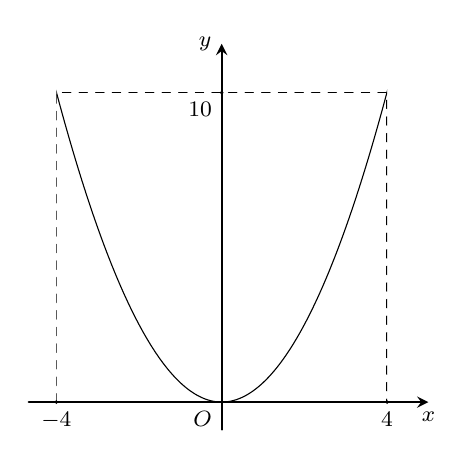
\begin{tikzpicture}[scale=0.7, font=\footnotesize, line join=round, line cap=round, >=stealth]
				\draw[->, line width=0.8pt](-3.5, 0)--(3.75, 0) node[below]{$x$};
				\draw[->, line width=0.8pt](0,-0.5)--(0,6.5) node[left]{$y$};
				\node at (0, 0) [below left]{$O$};
				\fill (3,0) node[below]{$4$} circle(1pt);
				\fill (-3,0) node[below]{$-4$} circle(1pt);
				\fill (0,5.6125) node[below left]{$10$} circle(1pt);
				\clip(-3,-0.1) rectangle(3,5.75);
				\draw[ smooth,samples=300] plot(\x,{5/8*(\x)^2});
				\draw[dashed] (-3,0)--(-3,5.6125)--(3,5.6125)--(3,0);
			\end{tikzpicture}
		}
	}
\end{ex}
\Closesolutionfile{ans}
% \indapan{6}{ans/ans-2-C4B13-D1-KQ}

